

Nesse capítulo, serão mostrados as técnicas utilizadas para a solução dos sistemas lineares gerados a partir da discretização apresentada no Capítulo \ref{ch:discretizacao}. Nas simulações reais de geomecânica, a quantidade de células pode chegar a centenas de milhões de elementos de forma que métodos efetivos de estruturas de dados e algoritmos são necessários para que a resolução seja possível. A Seção \ref{sec:csr} apresenta uma breve discussão sobre as estruturas de dados para armazenamento das matrizes, a Seção \ref{sec:cg} apresenta alguns métodos de solução de sistemas esparsos, enquanto que a Seção \ref{sec:fatoracaolu} apresenta a fatoração LU.


\section{Estruturas de Dados para Matrizes Esparsas} \label{sec:csr}

Conforme mostrado no Capítulo \ref{ch:discretizacao}, a quantidade de não zeros da matriz (nnz) é $O(\qtdnos)$, enquanto a quantidade total de entradas da matriz é da ordem de $O(\qtdnos^2)$. Dessa forma, é necessário utilizar uma estrutura de dados que seja capaz de apenas armazenar apenas os não zeros para torna o \textit{software} mais eficiente.  Uma ideia simples para guardar esse tipo de matriz consiste em guardar para cada elemento não zero seu valor, sua linha e sua coluna. Esse formato é chamado de \textit{Coordinate Format} (COO) mostrado em \citet{solverlinear}. Três vetores são necessários para guardar os valores:


\begin{itemize}
    \item JR: vetor que guarda a linha de cada entrada (Tamanho $nnz$)
    \item JC: vetor que guarda a coluna de cada entrada (Tamanho $nnz$)
    \item AA: vetor que guarda os valores das entrada (Tamanho $nnz$)
\end{itemize}


Assim a matriz


\begin{equation}
    \begin{bmatrix}
        1 & 0 & 2 & 0\\
        3 & 4 & 0 & 5\\
        0 & 6 & 7 & 0\\
        0 & 0 & 8 &9
    \end{bmatrix}
\end{equation}

Tem como vetores associados na sua representam COO os mostrados abaixo:


\begin{center}
    \begin{itemize}
        \item  JR = 1 1 2 2 2 3 3 4 4
        \item  JC = 1 3 1 2 4 2 3 3 4
        \item  AA = 1 2 3 4 5 6 7 8 9
    \end{itemize}
\end{center}


É importante perceber que nesse formato, as entradas da matriz podem ser escritas em qualquer ordem. Porém, no exemplo acima, elas estão ordenadas por linha e pode-se notar que o vetor JR apresenta uma série de valores repetidos. Para tirar proveito dessa repetição, existe outro formato chamado \textit{Compressed Row Format} (CSR) onde o vetor associado as linhas JR é substituido por um vetor IA que é um ponteiro para o vetor de colunas com o início de cada uma das linhas.

Para a matriz acima, tem-se:

\begin{itemize}
    \item A linha 1 é a primeira e, portanto, IA(1) = 1
    \item A linha 2 começa a partir do elemento 3 do vetor AA e, portanto, IA(2) = 3
    \item A linha 3 começa a partir do elemento 5 do vetor AA e, portanto, IA(3) = 6
    \item A linha 4 começa a partir do elemento 7 do vetor AA e, portanto, IA(4) = 8
\end{itemize}

É adicionado ainda um valor a mais ao vetor IA que guarda a quantidade de nnz+1. No exemplo acima, esse valor é  IA(5) = 10, com isso é possível saber as entradas de determinada linha $i$ olhando para as posições $IA(i)$ a $IA(i+1)-1$ do vetor AA e as respectivas colunas em JC. Os valores dos vetores CSR da matriz então ficam:

%TODO deixar valores one-based
\begin{center}
    \begin{itemize}
        \item IA = 1 3 7 8 10
        \item JA = 1 3 1 2 4 2 3 3 4
        \item AA = 1 2 3 4 5 6 7 8 9
    \end{itemize}
\end{center}


De acordo com \citet{solverlinear}, o formato CSR é provavelmente o mais comum mais popular para guardar matrizes esparsas e costuma ser a porta de entrada de estrutura de dados para matrizes esparsas. Nesse trabalho, a implementação é feita utilizando esse tipo de estrutura de dados conforme será mostrado no Capítulo \ref{ch:implementacao}.

Uma operação particularmente importante com as matrizes é a multiplicação matriz vetor $y = Ax$. No contexto dessa dissertação, ela é importante para aplicar o operadores de prolongamento e restrição apresentados no Capítulo \ref{ch:multiescala} e também nos métodos de solução de sistemas lineares Gradiente Conjugado (CG) e Bicgstab. O Algoritmo \ref{alg:algoritmomatmult} apresenta a multiplicação matriz vetor utilizando uma matriz CSR representada pelos vetores IA, JA, AA pelo vetor x.


\vspace{1cm}
\begin{algorithm}[H]
\caption{y = MultMatrizVetor(IA(n+1), JA(nnz), AA(nnz), x(n))}
\label{alg:algoritmomatmult}
\Inicio{

 y $\leftarrow \mathbf{0}$ 
 
\Para{row $\in$ \{1, 2, 3, ..., n\}}{
    \Para{j $\in$ \{IA(\text{row}), ..., IA(\text{row}+1)-1\}}{
        col $\leftarrow$ JA(j)
        
        y(row) $\leftarrow$ y(row) + AA(j) $\times$ x(col)
    }
}

}

\end{algorithm}
\vspace{1cm}


Nesse algoritmo, é importante perceber que a variável j irá assumir valores de 1 a IA(n+1)-1 e ,como IA(n+1)=$nnz + 1$, esse algoritmo tem que complexidade $O(nnz)$. 
O CSR então além de necessitar de menos memória para armazenar a matriz também tem a vantagem de fazer operações de multiplicação mais eficientemente visto que a complexidade seria $O(n^2)$ caso a matriz fosse armazenada densa.


\section{Solução de Sistemas Esparsos} \label{sec:cg}

Nessa seção serão apresentados alguma métodos para solução de sistemas lineares, em especial o gradiente conjugado que será utilizado para as comparações entre o método multiescala e multigrid apresentados no Capítulo \ref{ch:resultados}. Será considerado o sistema linear apresentado em \eqref{eq:sistemalinear4}.

\begin{equation} \label{eq:sistemalinear4}
    \mathbf{Ax = b}
\end{equation}

\subsection{Pré-condicionadores}

Define-se como número de condicionamento da matriz a Equação apresentada em \eqref{eq:condicionamento}, quanto maior o número de condicionamento mais próximo da matriz ser singular. As matrizes advindas de sistemas gerados pelas Equações \eqref{eq:edp_geomec_contorno} costumam ter números de condicionamentos elevados fazendo com que os métodos de solução tenham dificuldade de convergir.

\begin{equation} \label{eq:condicionamento}
1+1=2
\end{equation}


Uma estratégia importante para a solução desses sistemas lineares é a utilização de pré-condicionadores que consistem em tentar resolver um sistema equivalente a \eqref{eq:sistemalinear4} mas com um número de condicionamento menor. Há dois principais métodos de pré-condicionamento, pela esquerda ou pela direita. Chamando de $\mathbf{M}$ a matriz de pré-condicionamento  \eqref{eq:preconesq} e \eqref{eq:precondir} apresentam o pré-condicionamento pela esquerda e pela direita respectivamente. A matriz de pré-condicionamento geralmente aproxima a matriz original $\mathbf{A}$, de forma que $\precon \mathbf{A}$ e $\mathbf{A} \precon$ tenham número de condicionamento ordens de grandeza menores que o da matriz original. Um fato importante é que apesar de aparecerem os produtos $\precon \mathbf{A}$ e $\mathbf{A} \precon$ eles não efetivamente realizados, pois, muitas vezes se é conhecido apenas a matriz $\mathbf{M}$ e, mesmo que $\precon$ fosse conhecido, esses produtos podem ser densos.  


\begin{equation} \label{eq:preconesq}
\precon \mathbf{A} \mathbf{x}= \precon \mathbf{b}
\end{equation}

\begin{align} \label{eq:precondir}
\mathbf{A} \precon \mathbf{y} = \mathbf{b} \\
\mathbf{x} = \precon \mathbf{{y}}
\end{align}


Um pré-condicionador popular são os baseados em fatorações incompletas (ILU) apresentados em \citet{ilupaper}. Esses pré-condicionadores calculam aproximações para a fatoração LU de uma matriz e são apresentadas na seção \ref{sec:fatoracaolu}.

\subsection{Iteração de Richardson}

Um método simples de solução de sistemas lineares é a Iteração de Richardson, essa solução é utilizado em solvers multiescala apresentados em \citet{msparalelo}. No caso, dada a matriz uma matriz A e um pré-condicionador M uma iteração do método é definida conforme apresentado em \eqref{eq:iteracaorichardson}.

\begin{align} \label{eq:iteracaorichardson}
\mathbf{I}_m = (\mathbf{I} - \precon \mathbf{A})    \\
\mathbf{x}_{i+1} = \mathbf{I}_m  \mathbf{x}_i + \precon \mathbf{b}  
\end{align}

A partir de \eqref{eq:iteracaorichardson} é possível encontrar a equação do erro ao longo das iterações $e_{i+1} = \mathbf{I}_m e_i$, isso faz com que a convergência seja garantida apenas se $\rho(\mathbf{I}_m) < 1$, onde $\rho$ representa o raio espectral da matriz. Essa condição é necessária para que cada componente do erro relativa a um autovetor reduza a cada iteração.


\subsection{Método do Gradiente Conjugado}

O método dos Gradiente Conjugado pode ser utilizado na solução de sistemas lineares da forma \eqref{eq:sistemalinear4} onde $A$ é uma matriz simétrica positiva definida (SPD). Nesse caso, pode-se encontrar um problema de minimização equivalente através da definição da forma quadrática apresentada em \eqref{eq:quadratica}. 

\begin{equation} \label{eq:quadratica}
    f(\mathbf{x}) = \frac{1}{2}  \mathbf{x}^T \mathbf{A} \mathbf{x} - \mathbf{b}^T \mathbf{x} + c, \quad f:\mathbb{R}^n \rightarrow \mathbb{R}
\end{equation}

Para encontrar os pontos extremos da função \eqref{eq:quadratica} é necessário calcular os pontos em que o gradiente de $f$ é o vetor nulo. Portanto, é necessário calcular a derivada parcial de $f$ para cada uma das coordenadas. Para facilitar esse cálculo a equação \eqref{eq:quadratica} é apresentada em notação indicial em \eqref{eq:quadratica_ind}.


\begin{equation} \label{eq:quadratica_ind}
    f(\mathbf{x}) = \frac{1}{2} x_i A_{ij} x_j - b_i x_i + c_i
\end{equation}


Aplicando a derivada parcial com relação a uma coordenada $x_k$.


\begin{eqnarray}
     \dxk[f(\mathbf{x})] & = & \frac{1}{2} \dxk[ x_i A_{ij} x_j ]- \dxk{b_i x_i}+ \dxk{c_i} \\
                & = & \frac{1}{2} \dxk[ x_i A_{ij} x_j ]- b_k \\
                & = & \frac{1}{2} (\dxk[ x_i ]A_{ij} x_j  + x_i A_{ij} \dxk[x_j]) - b_k \\
                & = & \frac{1}{2}(A_{kj} x_j  + x_i A_{ik})  - b_k
\end{eqnarray}


Retornando para a notação matricial


\begin{equation}
    \nabla f = \frac{1}{2} (\mathbf{A}\mathbf{x} + \mathbf{A}^T \mathbf{x}) - \mathbf{b}
\end{equation}


\begin{equation}
    \nabla f = \frac{1}{2} (\mathbf{A} + \mathbf{A}^T) \mathbf{x} - \mathbf{b}
\end{equation}

Como $\mathbf{A}$ é simétrica ($\mathbf{A}^T = \mathbf{A}$)

\begin{equation} \label{eq:gradf}
    \nabla f = \mathbf{A} \mathbf{x} - \mathbf{b}
\end{equation}

Em um ponto extremo  $ \mathbf{x}_e$ de $f(\mathbf{x})$ tem-se $(\nabla f)|_{\mathbf{x}=\mathbf{x}_e} = 0 $

\begin{equation}
    \mathbf{A}\mathbf{x}_e - \mathbf{b} = 0
\end{equation}

\begin{equation}
    \mathbf{A}\mathbf{x}_e = \mathbf{b}
\end{equation}

Portanto, $f(\mathbf{x})$ possui um único ponto extremo $\mathbf{x}_e = \mathbf{A}^{-1}\mathbf{b}$ que é justamente a solução do sistema linear \eqref{eq:sistemalinear4}. Resta mostrar que $\mathbf{x}_e$ é um ponto de mínimo. A demonstração a seguir pode ser encontrada em \citet{Shewchuk94anintroduction}. Considerando $\mathbf{x} = \mathbf{x}_e + \mathbf{e}$ com $\mathbf{e} \neq 0 $


\begin{align}
     f(\mathbf{x}_e + \mathbf{e}) & =  \frac{1}{2} (\mathbf{x}_e + \mathbf{e})^T \mathbf{A} (\mathbf{x}_e + \mathbf{e}) - \mathbf{b}^T(\mathbf{x}_e + \mathbf{e}) + \mathbf{c}  \nonumber\\
                & =  \frac{1}{2} (\mathbf{x}_e^T\mathbf{A}\mathbf{x}_e + \mathbf{x}_e^T\mathbf{A}\mathbf{e} + \mathbf{e}^T\mathbf{A}\mathbf{x}_e + \mathbf{e}^T\mathbf{A}\mathbf{e} )- \mathbf{b}^T(\mathbf{x}_e + \mathbf{e}) + \mathbf{c}  \nonumber\\
                & =  \frac{1}{2} \mathbf{x}_e^T\mathbf{A}\mathbf{x}_e -\mathbf{b}^T\mathbf{x}_e + \mathbf{c} + \frac{1}{2} ( \mathbf{x}_e^T\mathbf{A}\mathbf{e} + \mathbf{e}^T\mathbf{A}\mathbf{x}_e + \mathbf{e}^T\mathbf{A}\mathbf{e} ) - \mathbf{b}^T\mathbf{e}  \nonumber\\
                & =  f(\mathbf{x}_e) + \frac{1}{2} ( \mathbf{x}_e^T\mathbf{A}\mathbf{e} + \mathbf{e}^T\mathbf{A}\mathbf{x}_e + \mathbf{e}^T\mathbf{A}\mathbf{e} ) - \mathbf{b}^T\mathbf{e}  \nonumber\\
                & =  f(\mathbf{x}_e) + \frac{1}{2} ( (\mathbf{A}^{-1}\mathbf{b})^T\mathbf{A}\mathbf{e} + \mathbf{e}^T\mathbf{A}\mathbf{A}^{-1}\mathbf{b} + \mathbf{e}^T\mathbf{A}\mathbf{e} ) - \mathbf{b}^T\mathbf{e}  \nonumber\\
                & =  f(\mathbf{x}_e) + \frac{1}{2} ( \mathbf{b}^T\mathbf{A}^{-1}\mathbf{A}\mathbf{e} + \mathbf{e}^T\mathbf{b} + \mathbf{e}^T\mathbf{A}\mathbf{e} ) - \mathbf{b}^T\mathbf{e}  \nonumber\\
                & =  f(\mathbf{x}_e) + \frac{1}{2} ( \mathbf{b}^T\mathbf{e} + \mathbf{e}^T\mathbf{b} + \mathbf{e}^T\mathbf{A}\mathbf{e} ) - \mathbf{b}^T\mathbf{e}  \nonumber\\
                & =  f(\mathbf{x}_e) + \frac{1}{2}  \mathbf{e}^T\mathbf{A}\mathbf{e}  + \mathbf{b}^T\mathbf{e} - \mathbf{b}^T\mathbf{e}  \nonumber\\
                & =  f(\mathbf{x}_e) + \frac{1}{2}  \mathbf{e}^T\mathbf{A}\mathbf{e} \nonumber
\end{align}


Como $\mathbf{A}$ é positiva definida pela definição $\mathbf{e}^T\mathbf{A}\mathbf{e}  > 0$, logo

\begin{equation}
    f(\mathbf{x}_e + \mathbf{e}) = f(\mathbf{x}_e) + \frac{1}{2}  \mathbf{e}^T\mathbf{A}\mathbf{e} > f(\mathbf{x}_e)\rightarrow  f(\mathbf{x}_e + \mathbf{e}) > f(\mathbf{x}_e) \forall \mathbf{e} \neq 0
\end{equation}


Assim, $\mathbf{x}_e$ é ponto de mínimo global de $f(\mathbf{x})$ e o problema de encontrar $\mathbf{x}$ tal que $\mathbf{A}\mathbf{x} = \mathbf{b}$ é equivalente a \textit{minimizar} $f(\mathbf{x})$. Para encontrar o mínimo de $f$ é possível utilizar o método de otimização do Gradiente Conjugado. O método consiste em partir de um ponto $\mathbf{x}_0$ e caminhar em direções conjugadas até que o mínimo local seja encontrado. Entende-se por direções conjugadas $\mathbf{d}_i$ e $\mathbf{d}_j$ tais que $\mathbf{d}_i^T\mathbf{A}\mathbf{d}_j=0$. 

O método do gradiente encontra a solução exata do sistema linear após n iterações, onde n é a dimensão da matriz, porém, este é utilizado como solver iterativo aproximado onde outro critério de parada é utilizado, como por exemplo, quando o resíduo da solução se torna menor que determinado valor. O Algoritmo \ref{alg:algoritmocg} apresenta o método do gradiente conjugado. 


\vspace{1cm}
\begin{algorithm}[H]
\caption{GradienteConjugado($\mathbf{A}$, $\mathbf{x}$, $\mathbf{b}$, $i_{max}$, $\epsilon$)}
\label{alg:algoritmocg}
\Inicio{

$i \leftarrow 0$

$\mathbf{r} \leftarrow \mathbf{b} - \mathbf{A}\mathbf{x}$

$\mathbf{d} \leftarrow \mathbf{r}$

$\delta_{new} \leftarrow \mathbf{r}^T\mathbf{r}$

$\delta_{0} \leftarrow \delta_{new}$

\Enqto{ $i  < i_{max}$ e $\delta_{new} > \epsilon^2\delta_0$ }{
    
    $\mathbf{q} \leftarrow \mathbf{A}\mathbf{d}$
    
    $\alpha \leftarrow \delta_{new}/\mathbf{d}^T\mathbf{q} $ 
    
    $\mathbf{x} \leftarrow \mathbf{x} + \alpha \mathbf{d} $
    
    $\mathbf{r} \leftarrow \mathbf{r} - \alpha \mathbf{q} $
    
    $\delta_{old} \leftarrow \delta_{new} $
    
    $\delta_{new} \leftarrow \mathbf{r}^T\mathbf{r} $
    
    $\beta \leftarrow \delta_{new}/\delta_{old}$
    
    $\mathbf{d} \leftarrow \mathbf{r} + \beta \mathbf{d}$
    
    $i \leftarrow i + 1$
}

}
\end{algorithm}
\vspace{1cm}


\subsubsection{Gradiente Conjugado Pré-Condicionado}


Uma dificuldade em se utilizar pré-condicionamento com o Gradiente Conjugado é que o método necessita que a matriz seja simétrica para garantir a convergência para a solução do sistema linear. Porém, se aplicarmos um pré-condicionador $\precon$ esquerda ou pela direita perde-se que a simetria da matriz. Para solucionar essa questão, o pré-condicionador é dividido no produto $\mathbf{E}\mathbf{E}^T = \mathbf{M}$ e é aplicado simultaneamente pela esquerda e pela direita conforme mostrado em \eqref{eq:esqdirpreconcg}. É importante notar que para que tal decomposição exista é necessário que a matriz seja simétrica, visto que, $\mathbf{M}^T = (\mathbf{E}\mathbf{E}^T)^T = (\mathbf{E}^T)^T \mathbf{E}^T = \mathbf{E}\mathbf{E}^T = \mathbf{M}$. Em \citet{Shewchuk94anintroduction} é mostrado que apesar  dessa decomposição, o método não precisa calcular explicitamente a matriz $\mathbf{E}$ conforme apresentado no Algoritmo \ref{alg:algoritmocgprecon}.


\begin{align} \label{eq:esqdirpreconcg}
(\mathbf{E}^{-1})\mathbf{A}(\mathbf{E}^{-T}) \mathbf{y} = \mathbf{E}^{-1}\mathbf{b} \\
\mathbf{x} = \mathbf{E}^{-T} \mathbf{y}
\end{align}





\vspace{1cm}
\begin{algorithm}[H]
\caption{GradienteConjugadoPrecon($\mathbf{A}$, $\mathbf{x}$, $\mathbf{b}$, $\precon$, $i_{max}$, $\epsilon$)}
\label{alg:algoritmocgprecon}
\Inicio{

$i \leftarrow 0$

$\mathbf{r} \leftarrow \mathbf{b} - \mathbf{A}\mathbf{x}$

$\mathbf{d} \leftarrow \precon \mathbf{r}$

$\delta_{new} \leftarrow \mathbf{r}^T\mathbf{r}$

$\delta_{0} \leftarrow \delta_{new}$

\Enqto{ $i  < i_{max}$ e $\delta_{new} > \epsilon^2\delta_0$ }{
    
    $\mathbf{q} \leftarrow \mathbf{A}\mathbf{d}$
    
    $\alpha \leftarrow \delta_{new}/\mathbf{d}^T\mathbf{q} $ 
    
    $\mathbf{x} \leftarrow \mathbf{x} + \alpha \mathbf{d} $
    
    $\mathbf{r} \leftarrow \mathbf{r} - \alpha \mathbf{q} $
    
    $s \leftarrow \precon \mathbf{r}$

    $\delta_{old} \leftarrow \delta_{new} $
    
    $\delta_{new} \leftarrow \mathbf{r}^T\mathbf{s} $

    $\beta \leftarrow \delta_{new}/\delta_{old}$
    
    $\mathbf{d} \leftarrow \mathbf{r} + \beta \mathbf{d}$
    
    $i \leftarrow i + 1$
}

}
\end{algorithm}
\vspace{1cm}


\subsection{Método Multigrid}

O método multigrid tem como ideia principal a resolução do solver linear utilizando um conjunto de operadores que representam versões mais grosseiras do operador inicial onde os níveis mais finos são responsáveis a reduzir os erros de alta frequência enquanto os níveis mais grosseiros reduzem as frequências mais baixas do erro conforme mostrado em \citet{multigridtutorial}. O nível mais grosso geralmente é resolvido com solver direito, pois a quantidade de variáveis é pequena. 

Apesar de inicialmente ter sido concebido com ideias geométricas onde o operador é calculado com base no grid, poucas fontes mostram implementações dessa versão, e o método ficou mais reconhecido por sua versão algébrica onde os operadores são montados apenas a partir das entradas da matriz. Em especial, nesse trabalho será realizada a comparação com a biblioteca PyAmg (\citet{OlSc2018}).


Entre os níveis são necessários operadores que levam os vetores de uma escala mais fina para uma escala mais grossa e vice-versa. O operador que leva um vetor de um grid fino para o grid grosso é chamado de restrição, enquanto um que leva de um nível mais grosso para um nível mais fino é chamado de pronlongamento. 


Iniciando com um exemplo de solver multigrid apenas com dois níveis, chamemos de $\mathbf{A^1}$ como sendo o operador do nível fino e $\mathbf{A}^2$ o operador do grid grosso. Nesse caso, só existe um operador de prolongamento ($\mathbf{P}_2^1$) e um operador de restrição ($\mathbf{R}^2_1$). Uma iteração de um solver multigrid com dois níveis é apresentado no Algoritmo \ref{alg:ciclomg2niveis}. A cada ciclo multigrid, $\upsilon_1$ relaxações são aplicadas no grid fino antes de descer para o nível mais grosso e $\upsilon_2$ são aplicadas após o retorno do grid grosso para o grid fino. Esse ciclo é semelhante ao apresentado para o método multiescala no Capítulo \ref{ch:multiescala} com a diferença que apenas uma relaxação é aplicada no método multiescala.


Quando mais que dois níveis são utilizados com o Multigrid, existem mais opções de ciclos possíveis. O ciclo mais simples é o ciclo V apresentado na Figura \ref{fig:ciclov}, onde se desce até o nível mais grosso e retorna para o nível mais fino formando uma figura de V. Uma variação desse ciclo é apresentada na Figura \ref{fig:ciclow}. Esses dois ciclos podem ser descritos de acordo com o Algoritmo \ref{alg:ciclomu}, onde para o ciclo V o temos de $\mu = 1$ enquanto para o ciclo W $\mu = 2$. É fácil perceber que o ciclo W possui mais relaxações e mais aplicações de operadores de restrição e prologamento e, portanto, possui um maior custo computacional.

\begin{figure}[h]
\center
\subfigure[ Ciclo V ]{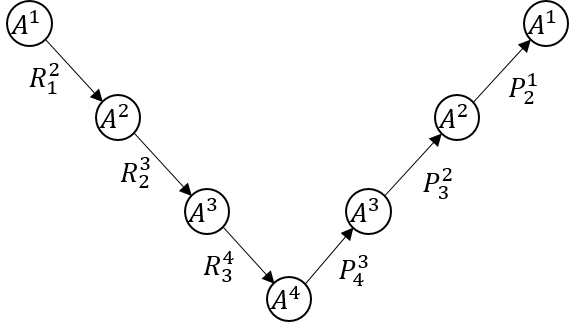
\includegraphics[width=0.5\textwidth]{chap04/figs/cicloV.png} \label{fig:ciclov}}
\qquad
\subfigure[Ciclo W ]{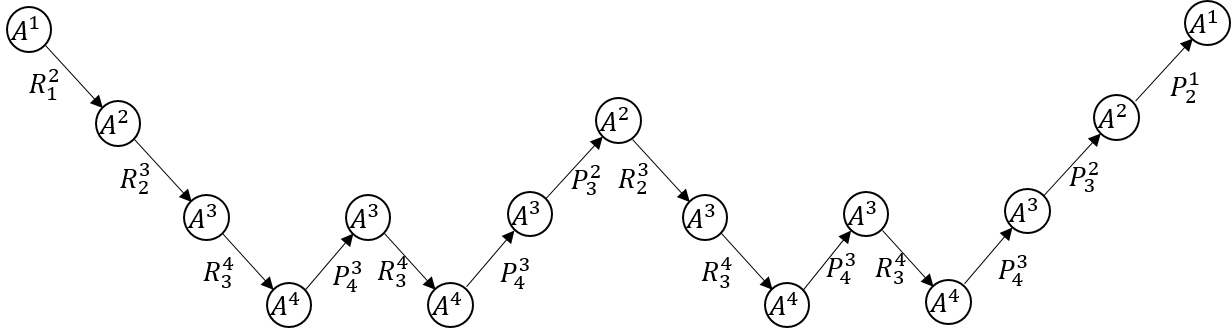
\includegraphics[width=0.8\textwidth]{chap04/figs/cicloW.png} \label{fig:ciclow}}
\caption{Aplicação de um ciclo V com dois níveis. Os círculos $A_1$, $A_2$, $A_3$ representam relaxações com esses operadores, enquanto o círculo relacionado a $A_4$ representa a solução direta de um sistema linear. }\label{fig:exemplomultigrid}
\end{figure}




\begin{algorithm}[H]
\caption{Ciclo-V($A_1$, $A_2$, $x_0$, $b$)}
\label{alg:ciclomg2niveis}
\Inicio{

$x_0 \leftarrow \text{relaxação}(A_1, x_0, b)$, $\upsilon_1$ vezes

$r \leftarrow b - A_1 x_0$

$r \leftarrow R^2_1 r$

$\delta_2 \leftarrow A_2^{-1} r$

$\delta_1 \leftarrow P^1_2 \delta_2$

$x_0 \leftarrow x_0 + \delta_1$

$x_0 \leftarrow \text{relaxação}(A_1, x_0, b)$, $\upsilon_2$ vezes
}

\end{algorithm}

\vspace{1cm}
\begin{algorithm}[H]
\caption{Ciclo-$\mu$($i$, $\mu$, $x$, $b$, $A_1$, $A_2$, ...) (Adaptado de \cite{multigridtutorial})}
\label{alg:ciclomu}
\Inicio{

$\text{relaxação}(A_i, x)$, $\upsilon_1$ vezes

$b_i \leftarrow R^{i+1}_i (b - A_i x)$


\Se{i + 1 é o nível mais grosso}{
    $x_{i+1} \leftarrow A_i^{-1} f$
}
\Senao{
    $x_{i+1} \leftarrow \mathbf{0}$

    $x_{i+1} \leftarrow x_{i+1} $ Ciclo-$\mu$($i+1$, $\mu$, $x_i$, $b_i$, $A_1$, $A_2$, ...), $\mu$ vezes
}

$x \leftarrow  x + P^i_{i+1} x_{i+1}$

$\text{relaxação}(A_i, x)$, $\upsilon_2$ vezes
}

\end{algorithm}
\vspace{1cm}


\subsubsection{Relaxações}


Em relação as relaxações utilizadas pelo método multigrid, duas relaxações bastante utilizadas são a Jacobi e o Gauss-Seidel. Elas tem como intuito remover os erros de alta frequência em cada um dos níveis multigrid. Em particular, a relaxação de Gauss Seidel simétrica foi utilizada na comparação do Capítulo \ref{ch:resultados} e é mostrada no Algoritmo \ref{alg:gauss_seidel}. É importante notar que, nesse caso a quantidade de operaçãoes feitas é proporcional a duas vezes o número de não zeros da matriz , pois, a relaxação é realizada começando de i=1 e depois voltando de i=n.

\vspace{1cm}

\begin{algorithm}[H]
\caption{Gauss-Seidel-Simétrico(A, x, b)}
\label{alg:gauss_seidel}
\Inicio{

$n \leftarrow \text{Tamanho de } A$

\Para{ $i \in 1,2,3,\cdots,n$}{
    \Para{$j \in 1,2,3,\cdots,n$}{
        $x(i) \leftarrow b(i)$
        
        \Se{$j \ne i$}{
            $x(i) \leftarrow x(i) - A(i,j) \times x(j)$
        }
    }
    $x(i) \leftarrow x(i)/A(i,i)$
}

\Para{ $i \in n,n-1,n-2,\cdots,1$}{
    \Para{$j \in 1,2,3,\cdots,n$}{
        $x(i) \leftarrow b(i)$
        
        \Se{$j \ne i$}{
            $x(i) \leftarrow x(i) - A(i,j) \times x(j)$
        }
    }
    $x(i) \leftarrow x(i)/A(i,i)$
}
}
\end{algorithm}

\vspace{1cm}


\subsubsection{Complexidade do Grid}
 
A implementação PyAmg nos seus solvers multigrid possui a medida de Complexidade do Grid, esse valor tenta representar o quão mais custoso é a utilização de um determinado solver multigrid em relação ao operador original. A definição desse valor é mostrado em \eqref{eq:complexidadegrid}. Como pode-se ver, ele conta quantos não zeros o somatório de todos os níveis possui a mais que o nível fino. Assim, por exemplo, considerando $\upsilon_1=1$ e $\upsilon_2=1$ cada nível irá realizar duas relaxações, com exceção do nível mais grosso, tornando o  custo de um ciclo aproximadamente $2\times\text{Complexidade Grid}$. 

\begin{equation}\label{eq:complexidadegrid}
    \text{Complexidade Grid} = \frac{\sum_{i=1}^n \text{nnz}(A_i)}{\text{nnz}(A_1)}
\end{equation}

Para saber o custo de um ciclo W se torna mais complicado devido a recursão associada a esse tipo de ciclo. No caso do ciclo apresentado na Figura \ref{fig:ciclow}, o operador $A_1$ são feitas duas relaxações o operador $A_2$ são feitas quatro relaxações (o vértice $A_2$ do meio em que chega e sai uma seta acontecem duas relaxações) e $A_3$ são feitas oito relaxações. O PyAmg também tem uma medida de complexidade do ciclo que é medida através de recursão e foi utilizada para as comparações que são apresentadas no Capítulo \ref{ch:implementacao}. 

%Primeiramente, é possível encontrar o ponto de mínimo ao de caminhar a partir ponto inicial $x_0$ e uma direção $d_0$. Dessa forma, sendo $x_1 = x_0 + \alpha d_0$ para encontrar o ponto que minimiza o $f(x_1)$ deve-se ter $\frac{d f(x_1)}{d\alpha} = 0$.

%\begin{equation}
%    \frac{df(x_1)}{d \alpha} =  \nabla f(x_1)^T d_0 = 0
%\end{equation}

%Pela equação \ref{eq:gradf}, $\nabla f(x_1) = -r_1 $ então:


% \begin{align}
%      r_1^T r_0                         & =  0 \\
%      r_0^T r_1                         & =  0 \\
%      r_0^T (b - Ax_1)                  & =  0 \\
%      r_0^T (b - A(x_0 - \alpha d_0))   & =  0 \\
%      r_0^T (b - Ax_0  - \alpha A d_0)  & =  0 \\
%      r_0^T (r_0 - \alpha A d_0)        & =  0 \\
%      r_0^T r_0 - \alpha  r_0^T A d_0   & =  0 \\
%      \alpha  r_0^T A d_0               & =  r_0^T r_0 \\
%      \alpha                            & =  \frac{r_0^T r_0}{r_0^T Ad_0}
% \end{align}

% O método dos gradientes conjugados em andar em direções conjugadas a cada passo de tempo minimizando $f(x)$ naquela direção. A direção inicial escolhida é

\section{Fatoração LU} \label{sec:fatoracaolu}

Outra parte importante para esse trabalho é a solução direta de sistemas, em particular por conta dos sistemas que serão resolvidos nos espaços grossos e também para cálculo das funções de base que serão apresentados no Capítulo \ref{ch:multiescala}. Esses sistemas tem um número reduzido de variáveis em comparação com os sistemas associados com o grid fino e, portanto, pode-se pensar na utilização de solvers diretos.

A fatoração LU consiste em transformar a matriz A em o produto de outras duas $\mathbf{A}=\mathbf{L}\mathbf{U}$: $\mathbf{L}$ triangular inferior e $\mathbf{U}$ triangular superior. Assim, o sistema fica da forma $\mathbf{L} \mathbf{U} \mathbf{x} = \mathbf{b}$ e a solução é realizada através da solução de dois sistemas triangulares $\mathbf{L}\mathbf{y} = \mathbf{b}$ e $\mathbf{U}\mathbf{x} = \mathbf{y}$. O cálculo dos fatores LU pode ser feita utilizando uma eliminação gaussiana e pode ser encontrado em \citet{heath1997scientific}. Uma vantagem desse método é que se for necessário resolver sistemas para diferentes lados direito $\mathbf{b}$ a fatoração pode ser reutilizada e não precisa ser calculada novamente. Para matrizes simétricas positivas definidas, existe a fatoração de Cholesky, similar a fatoração LU, onde $\mathbf{A} = \mathbf{L}^T \mathbf{L}$.


\subsubsection{Pré-condicionador ILU}

Os pré-condicionadores baseados em fatoração incompletas (ILU) apresentados em \citet{ilupaper} calculam uma aproximação para a fatoração LU da matriz. A aproximação é realizada desconsiderando algumas entradas das matrizes $\mathbf{L}$ e $\mathbf{U}$. Um parâmetro do método é o nível do ILU que controla a quantidade de entradas que a fatoração incompleta possui, em casos que o nível é zero a fatoração possui não zeros nas mesmas posições em que a matriz $\mathbf{A}$ possui entradas não-nulas. 
